\subsubsection{Biểu đồ thời gian chạy}

\textbf{3.2.1.1. Dữ liệu ngẫu nhiên}

Từ hình \ref{fig:randomize_running_time}, dễ thấy các thuật toán cơ bản có thời gian chạy lớn hơn rất nhiều so với các thuật toán còn lại. Bubble Sort có thời gian chạy chậm nhất (đường màu xanh). Shaker Sort là phiên bản cải tiến của Bubble Sort, có thời gian chạy tương đối tốt hơn Bubble Sort một chút. 4 thuật toán này có thời gian chạy tăng mạnh khi kích thước dữ liệu lớn hơn (bộ dữ liệu lên đến 500.000 phần tử). Điều này phù hợp với độ phức tạp $O(n^2)$ của chúng.


Các thuật còn lại bao gồm Shell Sort, Heap Sort, Merge Sort, Quick Sort, Counting Sort, Radix Sort, Flash Sort do thời gian chạy nhỏ nên các đường biểu diễn của chúng bị đè lên nhau thành một đường duy nhất (đường màu đỏ tía). Tiến hành loại bỏ 4 thuật toán cơ bản có thời gian chạy lớn, được hình \ref{fig:randomize_running_time_filtered}.

\begin{figure}[H]
    \centering
    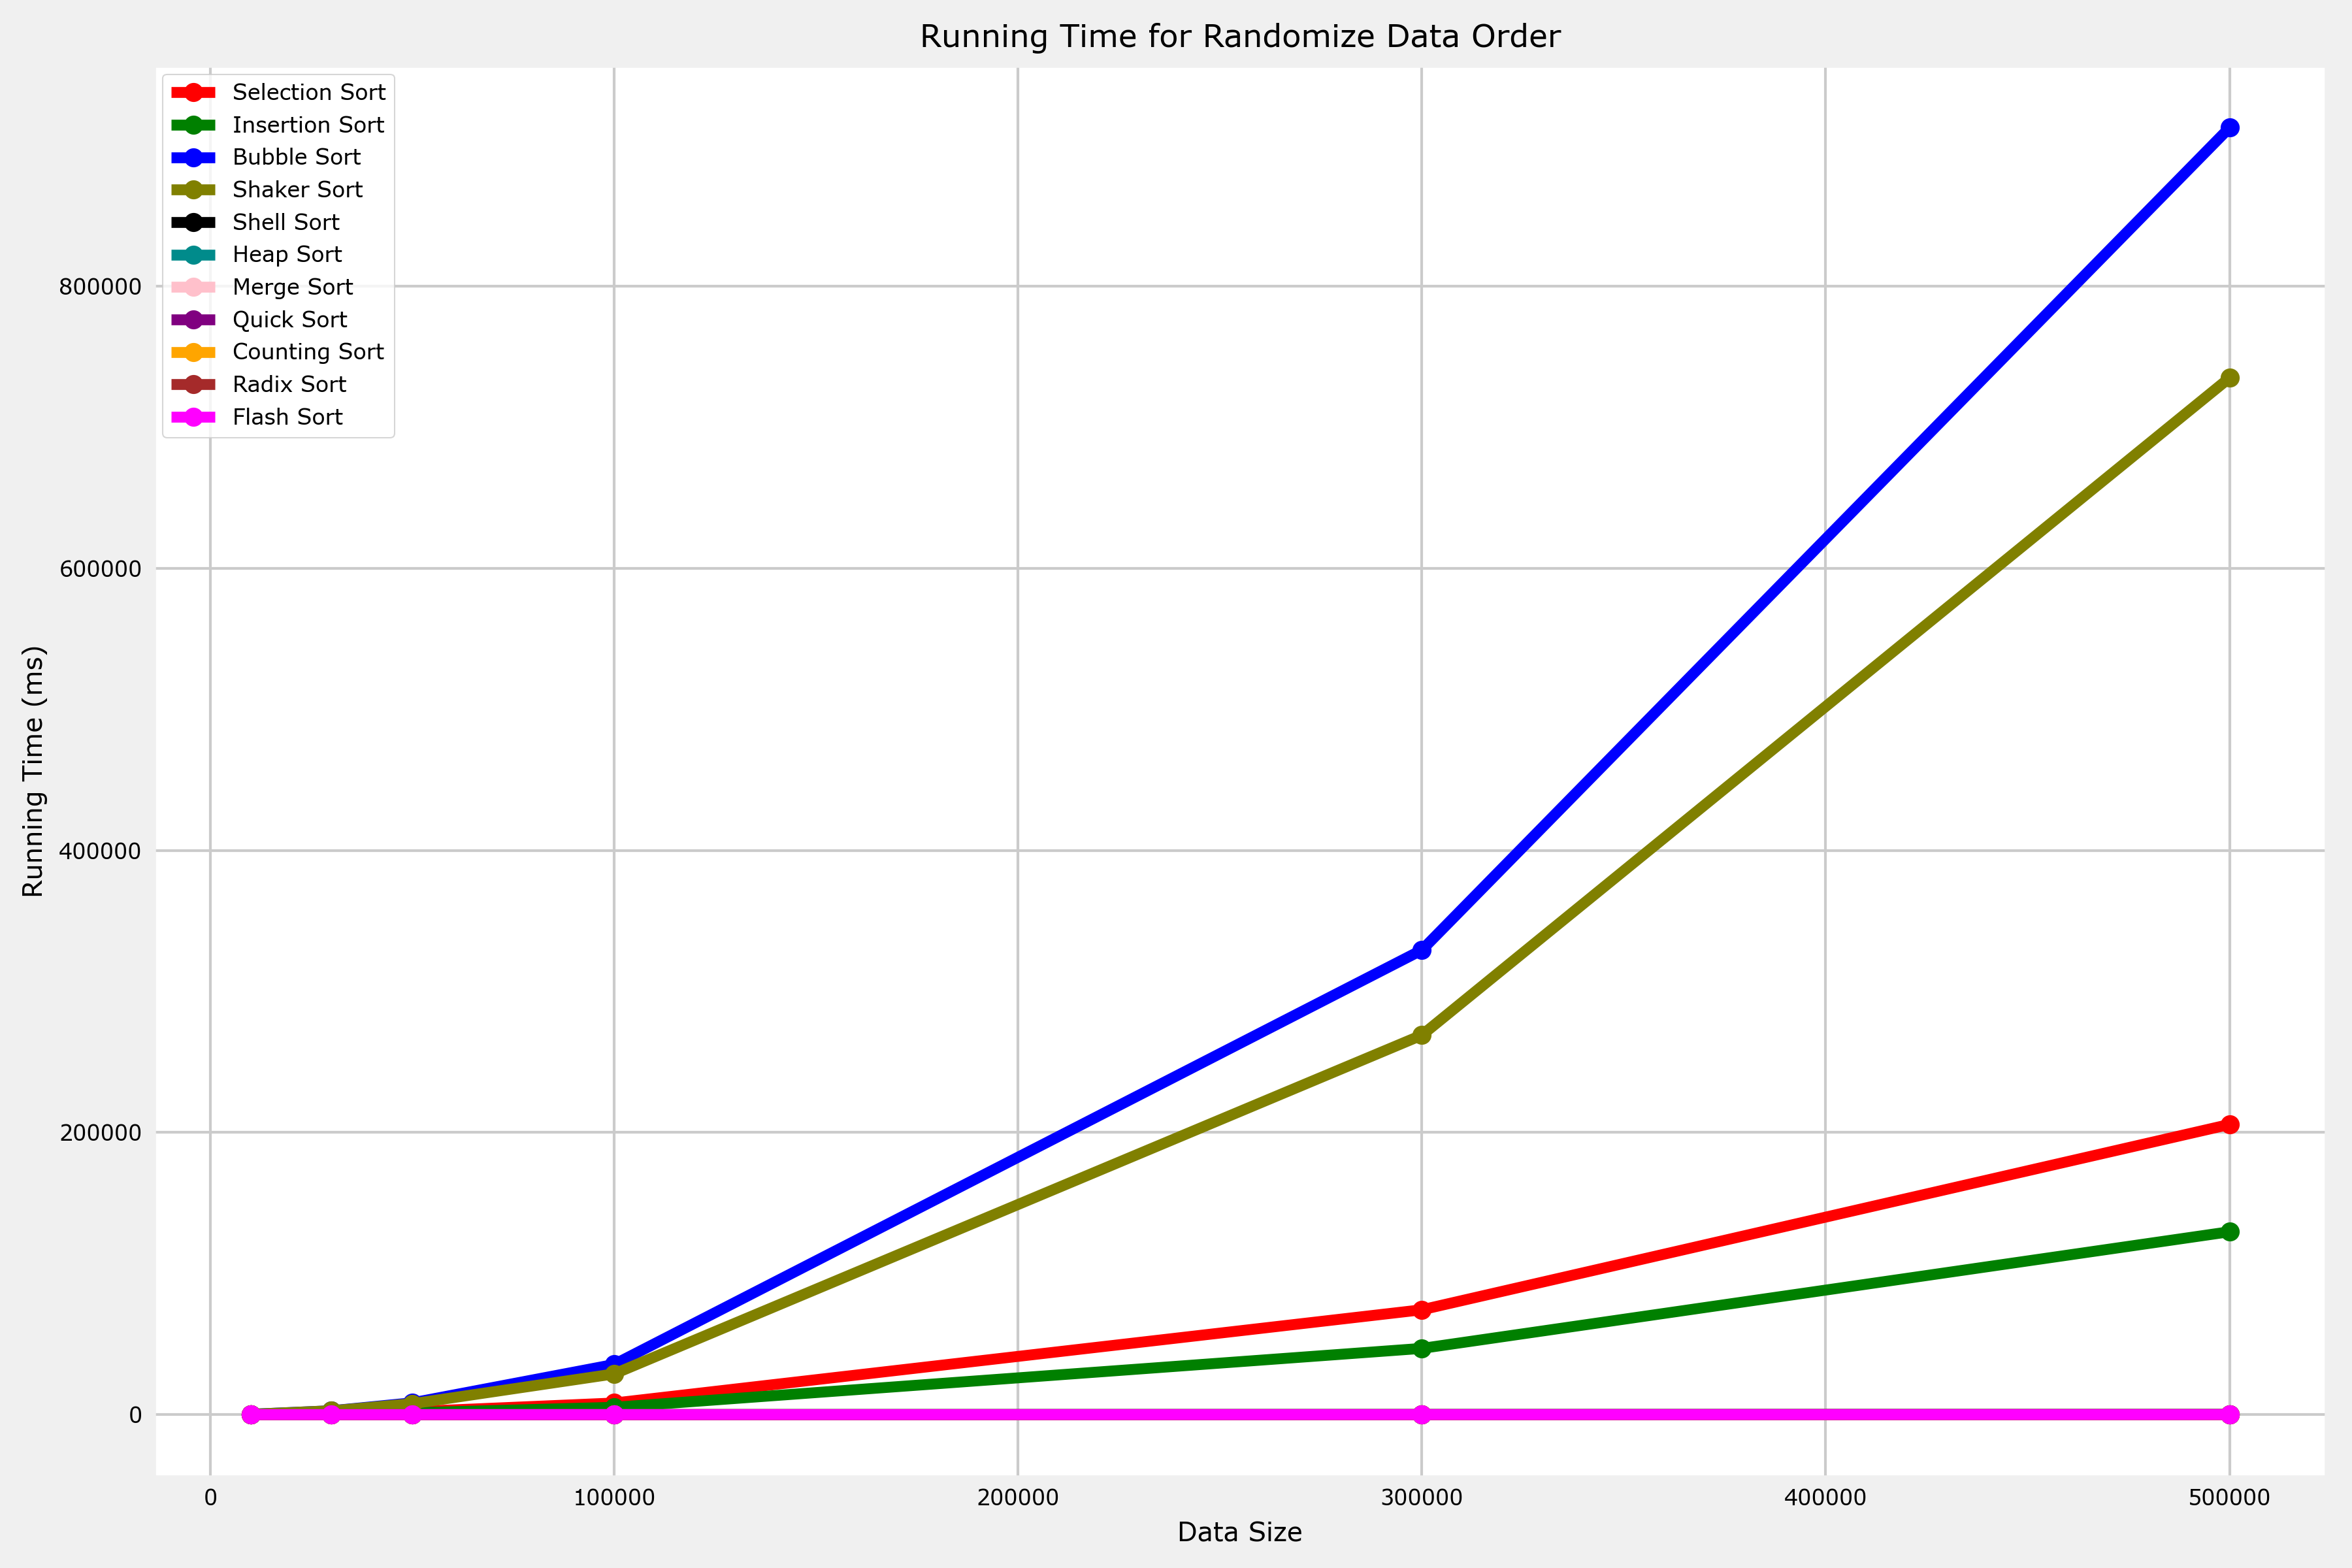
\includegraphics[width=\textwidth]{experimental_result/images/randomize_running_time.png}
    \caption{Thời gian chạy của 11 thuật toán với dữ liệu ngẫu nhiên}
    \label{fig:randomize_running_time}
\end{figure}


\begin{figure}[H]
    \centering
    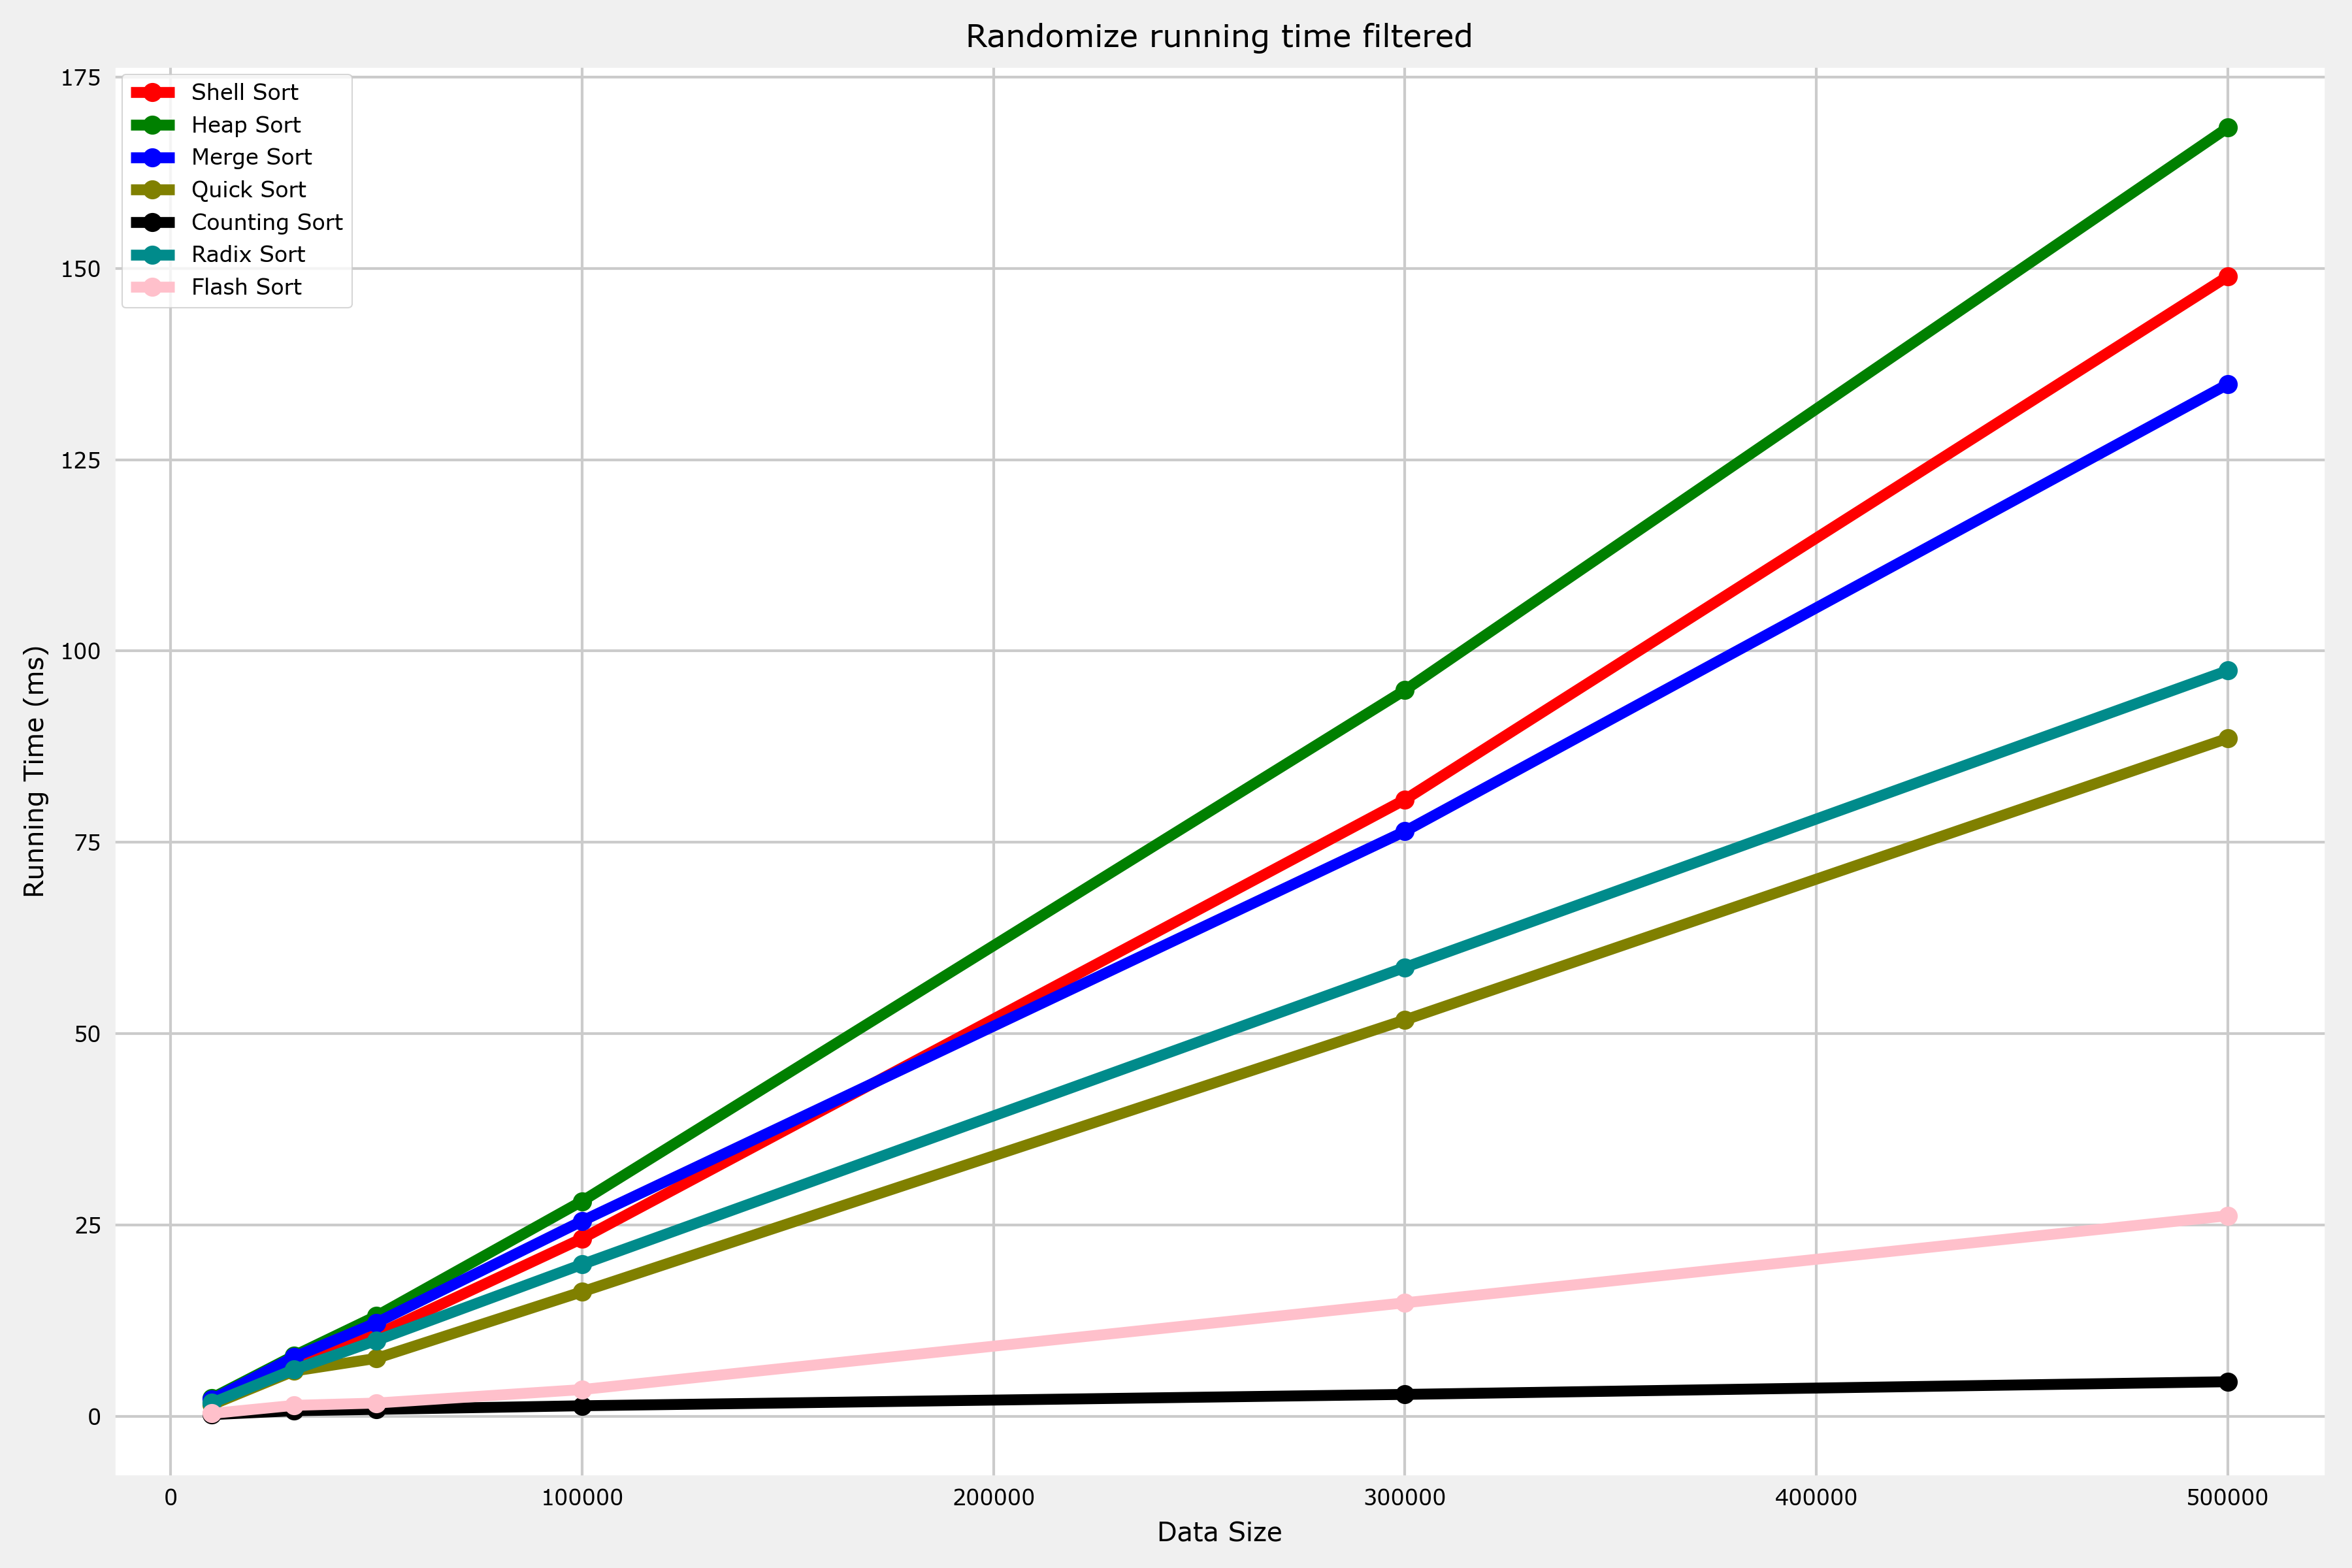
\includegraphics[width=\textwidth]{experimental_result/images/randomize_running_time_filtered.png}
    \caption{Thời gian chạy của 11 thuật toán với dữ liệu ngẫu nhiên sau khi loại bỏ outlier}
    \label{fig:randomize_running_time_filtered}
\end{figure}

Các thuật toán này có xu hướng tuyến tính hơn so với nhóm trước. Thuật toán Counting Sort và Flash Sort là hai thuật toán nhanh nhất, trong khi nhóm các thuật toán cải tiến có thời gian chạy cao hơn nhưng vẫn ổn định. Đặc biệt, Counting Sort có thời gian chạy rất nhỏ các tất cả trường hợp, đều bé hơn $5 ms$ (đường màu đen nằm rất gần trục hoành).




\begin{figure}[H]
    \centering
    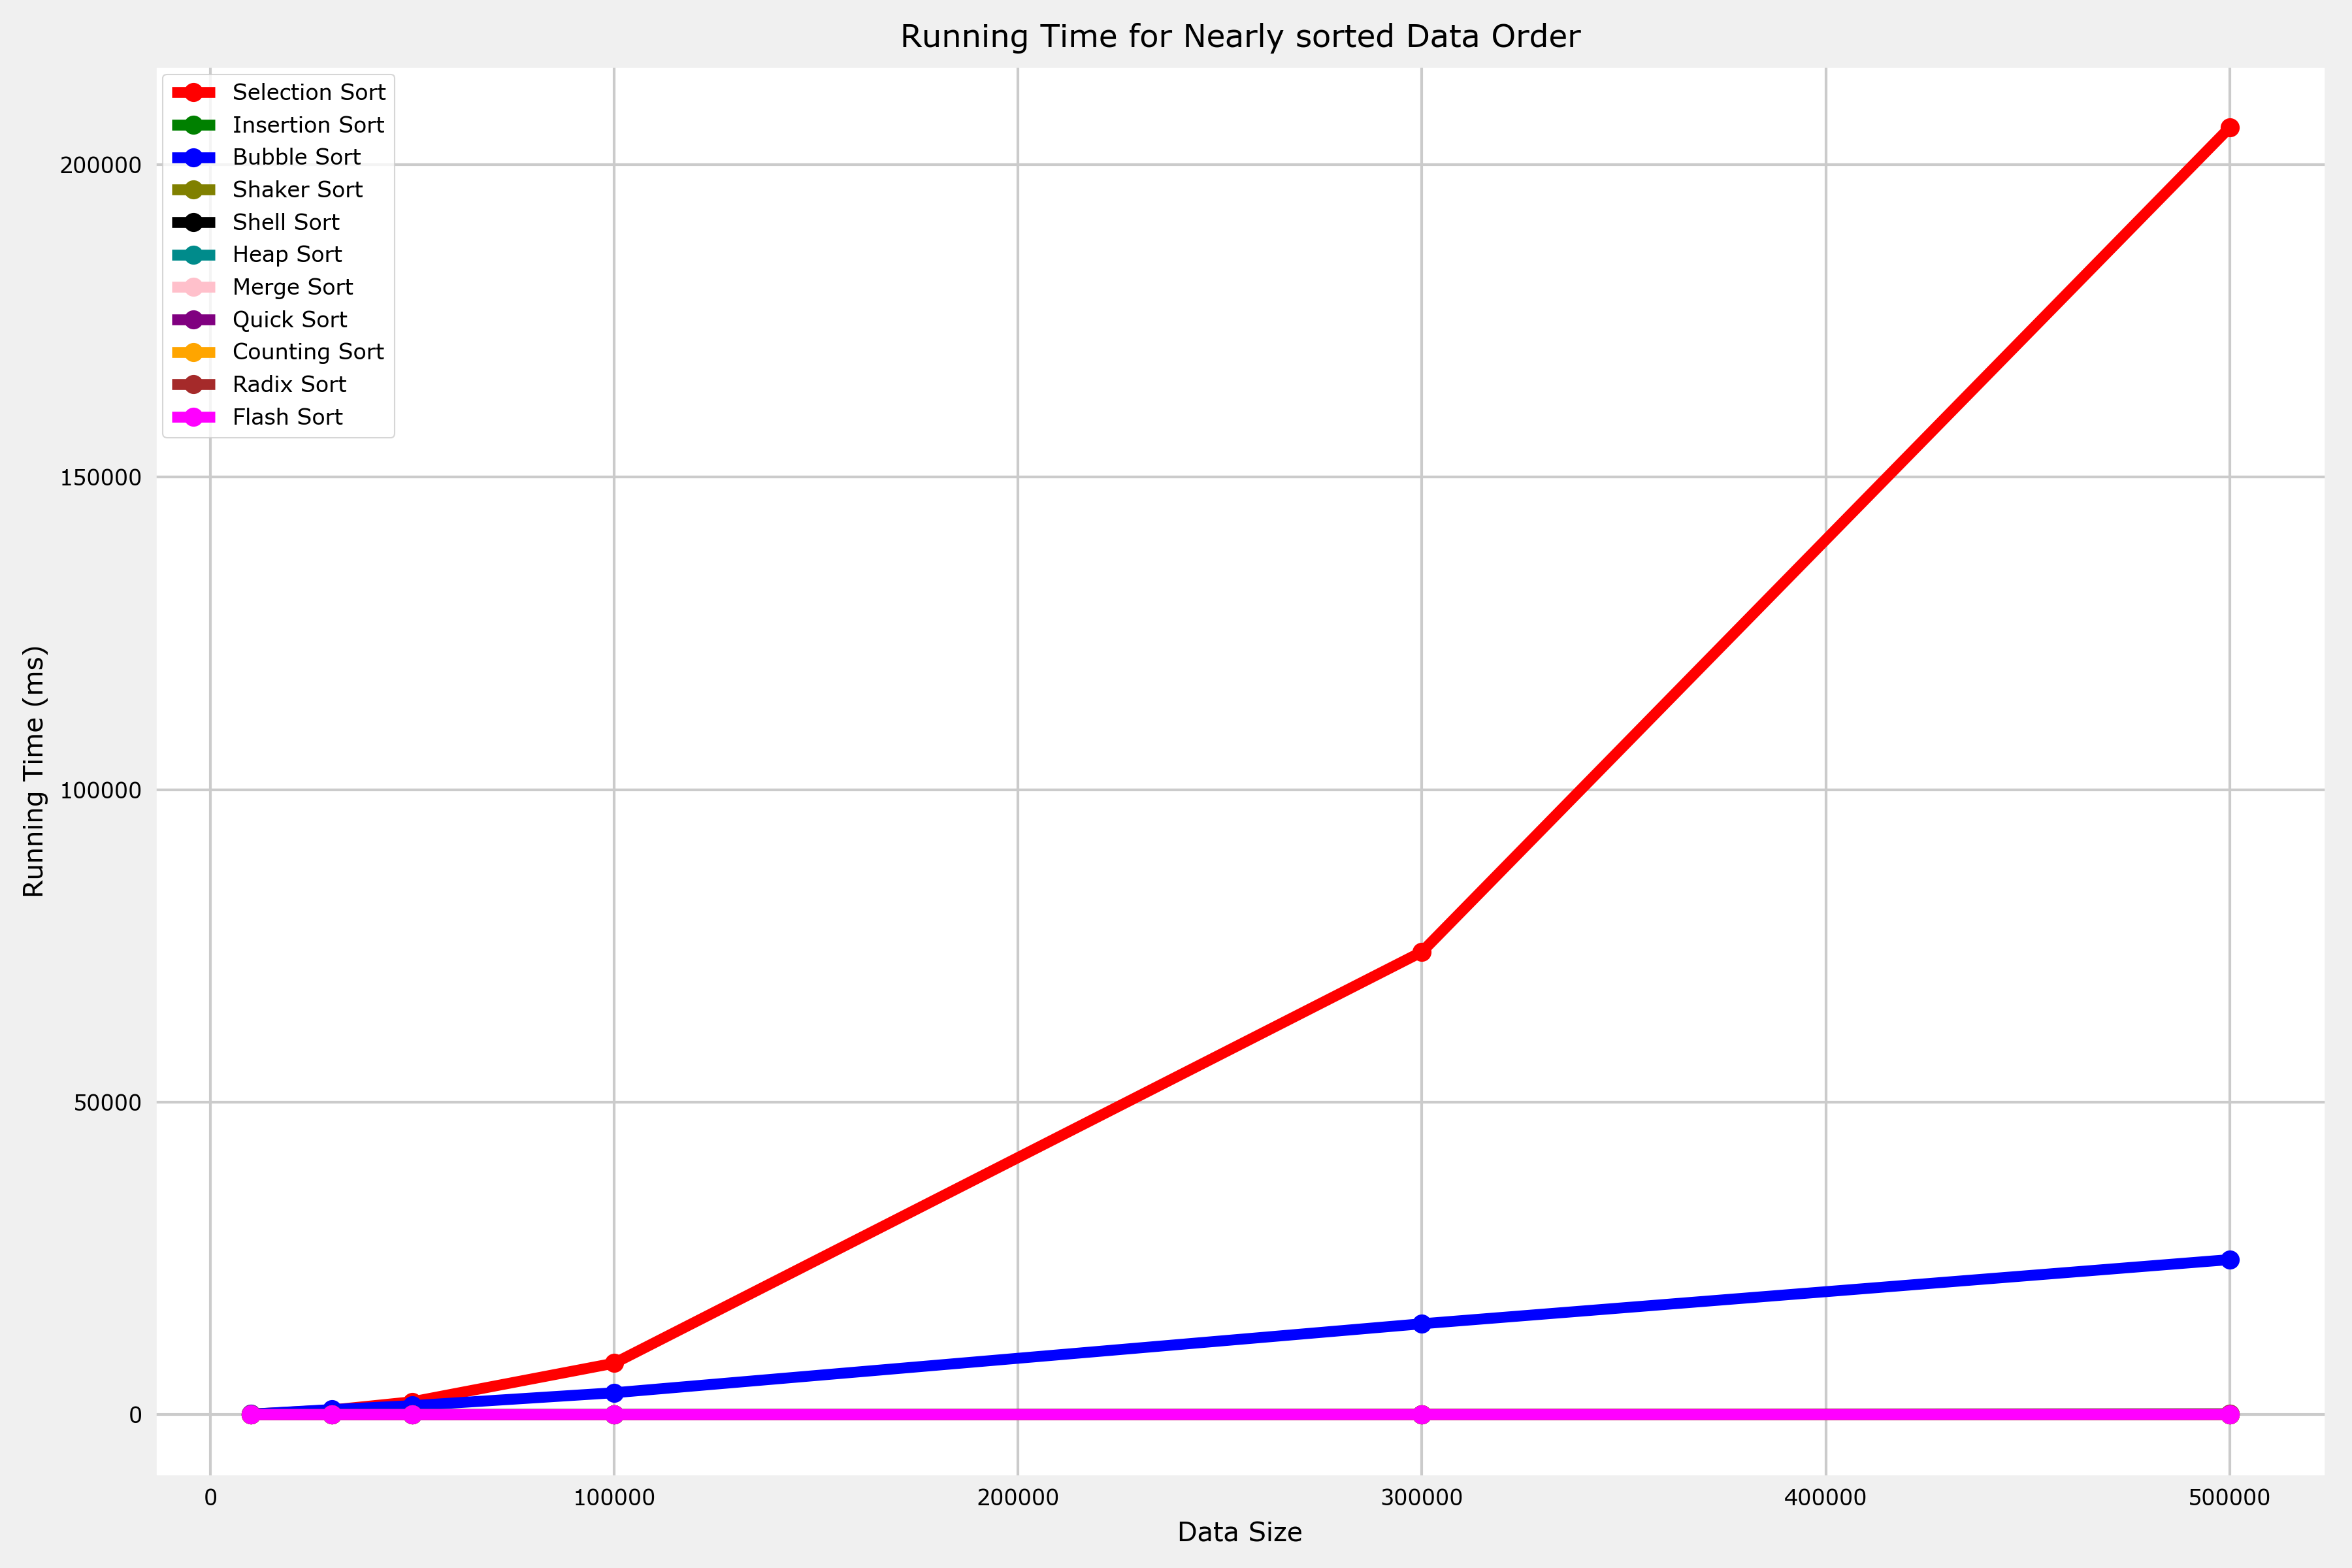
\includegraphics[width=\textwidth]{experimental_result/images/nearly_sorted_running_time.png}
    \caption{Thời gian chạy của 11 thuật toán với dữ liệu gần sắp xếp hoàn chỉnh}
    \label{fig:nearly_sorted_running_time}
\end{figure}
\textbf{3.2.1.2. Dữ liệu gần sắp xếp hoàn chỉnh}


Selection Sort có màn thể hiện rất tệ với dữ liệu gần sắp xếp hoàn chỉnh. Hình \ref{fig:nearly_sorted_running_time} thể hiện rõ độ phức tạp $O(n^2)$ của Selection Sort, tăng rất mạnh khi kích thước dữ liệu lên tới 500.000 phần tử. Thời gian chạy của Bubble Sort tốt hơn Selection Sort nhưng vẫn không tốt bằng các thuật toán khác. Các thuật toán còn lại không thể nhìn thấy do thời gian chạy của chúng nhanh hơn rất nhiều so với Selection Sort. Tiến hành loại bỏ Selection Sort và Bubble Sort, kết quả như hình \ref{fig:nearly_sorted_running_time_filtered}.


\begin{figure}[H]
    \centering
    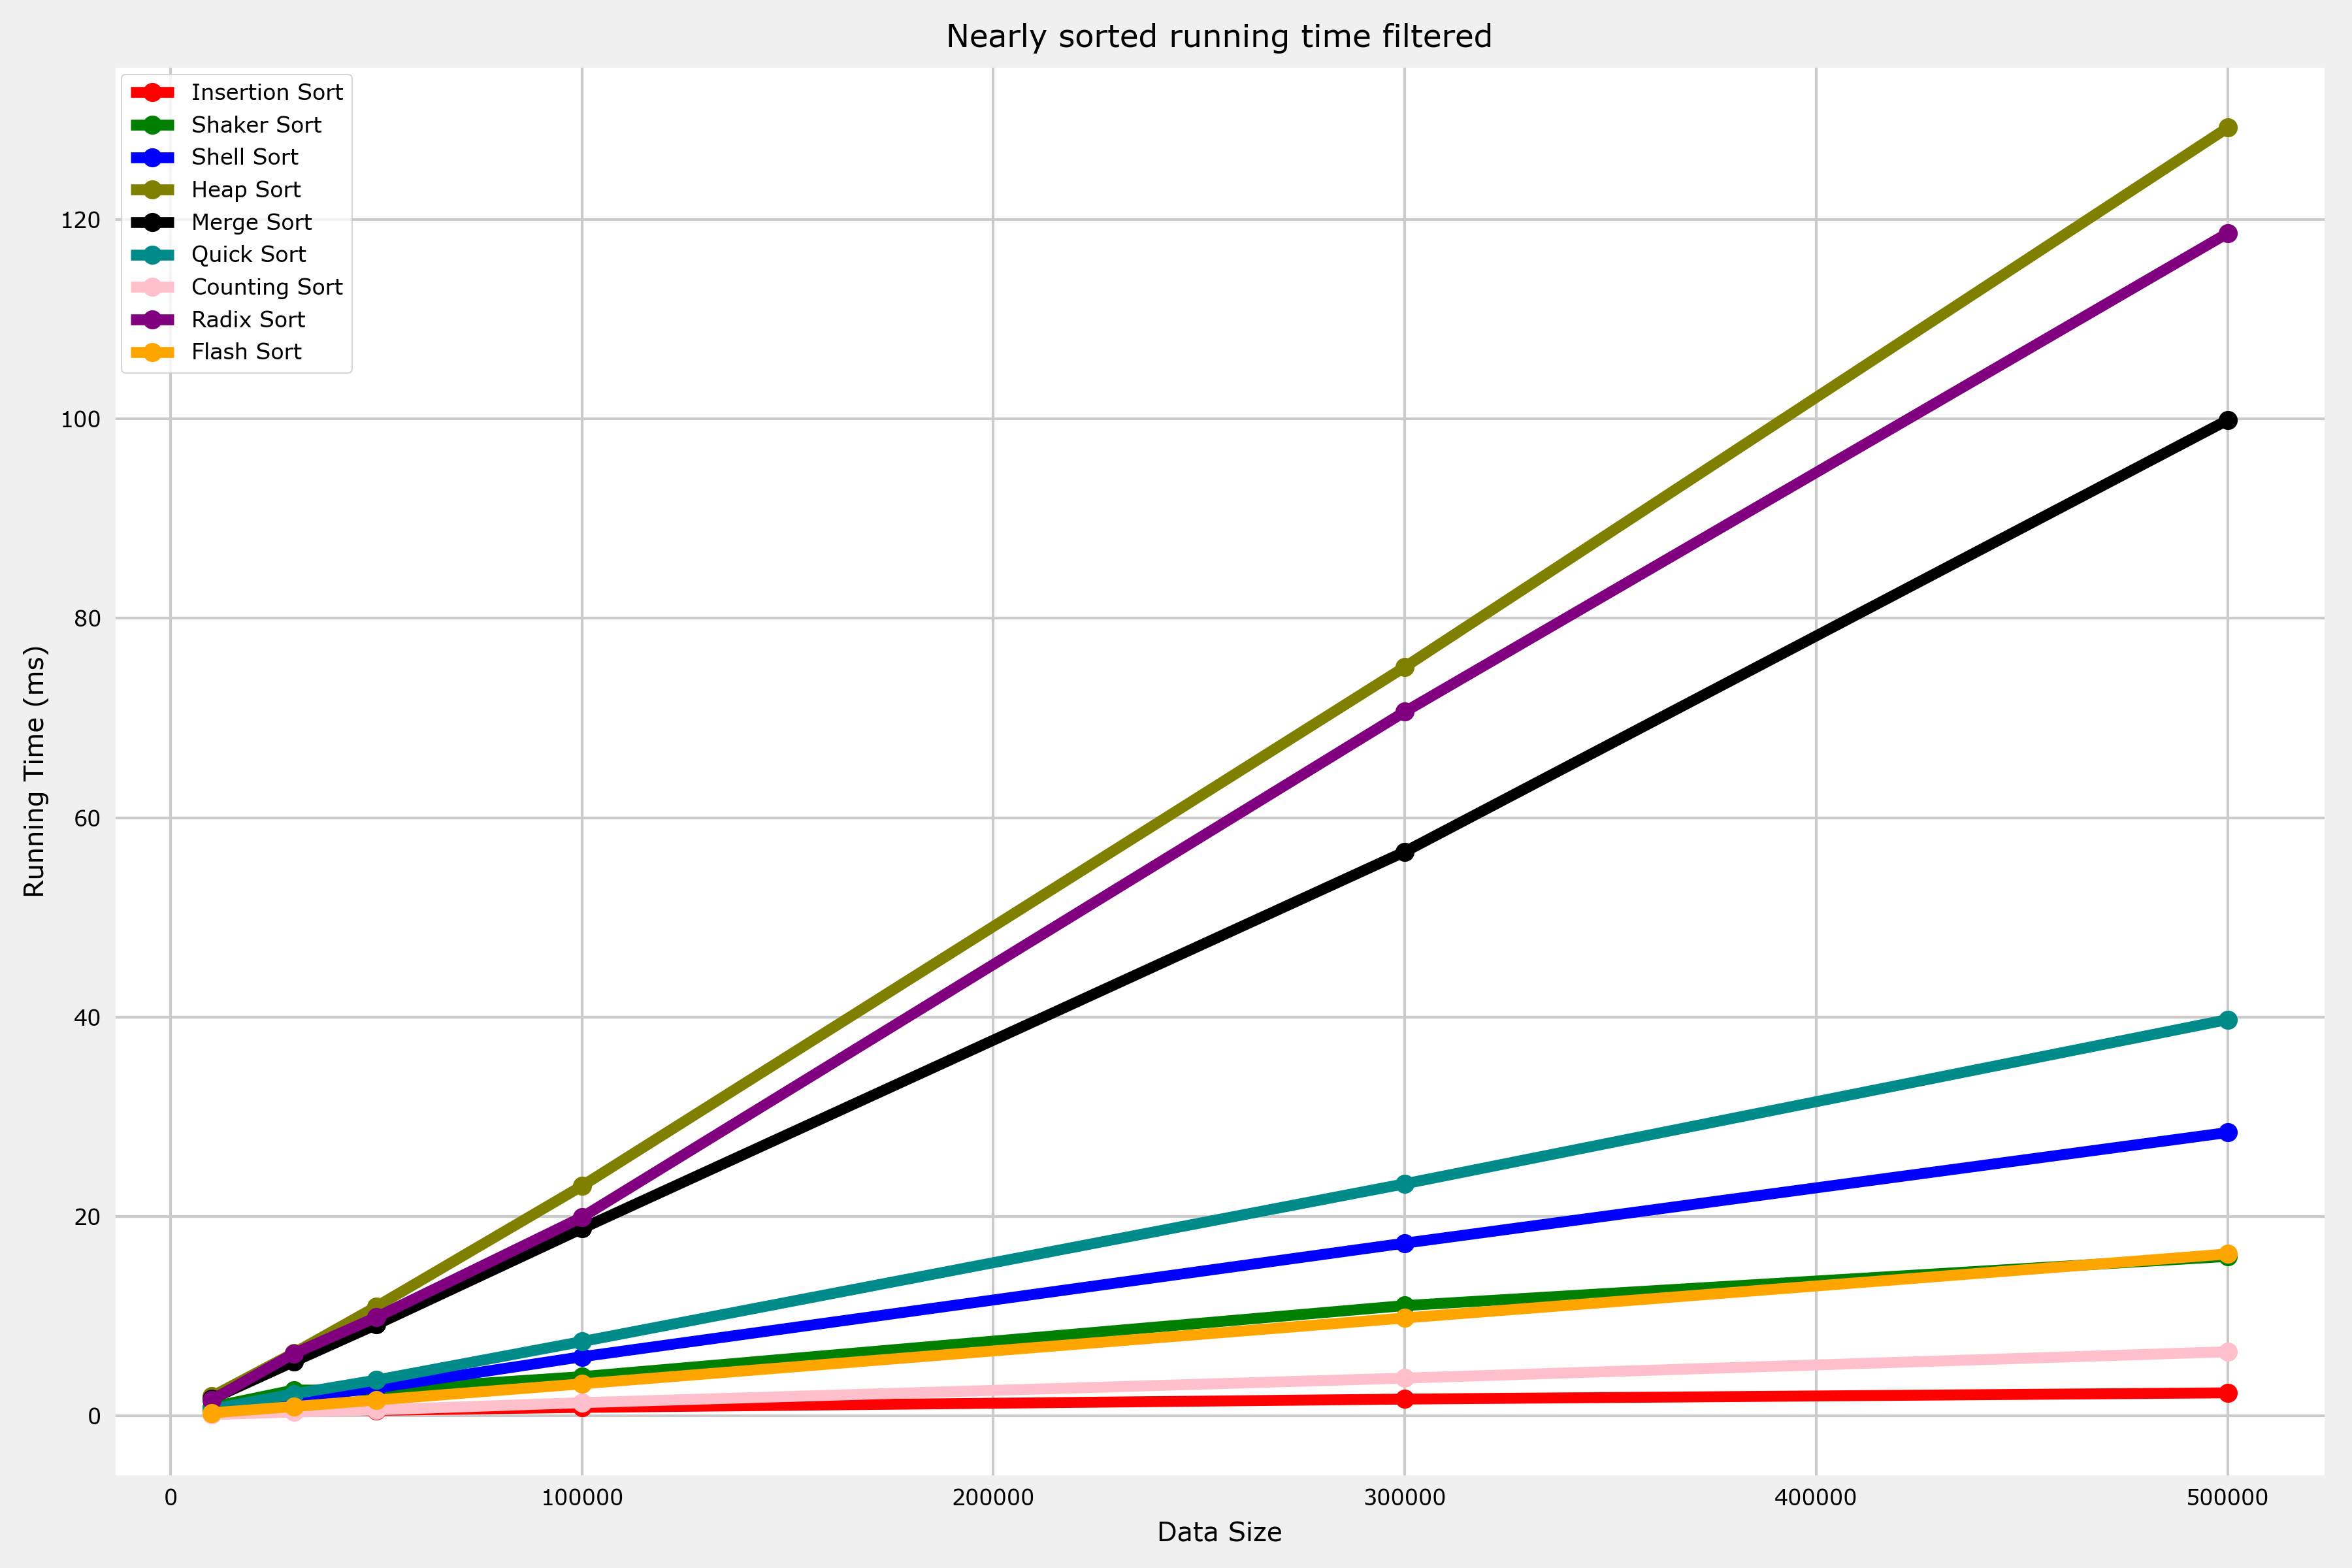
\includegraphics[width=\textwidth]{experimental_result/images/nearly_sorted_running_time_filtered.png}
    \caption{Thời gian chạy của 11 thuật toán với dữ liệu gần sắp xếp hoàn chỉnh sau khi loại bỏ outlier}
    \label{fig:nearly_sorted_running_time_filtered}
\end{figure}

Biểu đồ \ref{fig:nearly_sorted_running_time_filtered} lúc này có xu hướng chia thành hai nhóm nhóm 1 (Heap Sort, Radix Sort, Merge Sort) và nhóm 2, nhanh hơn (Quick Sort, Shell Sort, Shaker Sort, Flash Sort, Counting Sort, Insertion) .Insertion Sort có thời gian thực thi nhanh nhất với bộ dữ liệu này. Điều này khá phù hợp với trường hợp tốt nhất của Insertion Sort là dữ liệu đã sắp xếp. Shaker Sort tốt hơn nhiều so với Bubble Sort và xấp xỉ Flash Sort. Các thuật toán cải tiến và không sắp xếp khá ổn định giống như bộ dữ liệu trước.



\begin{figure}[H]
    \centering
    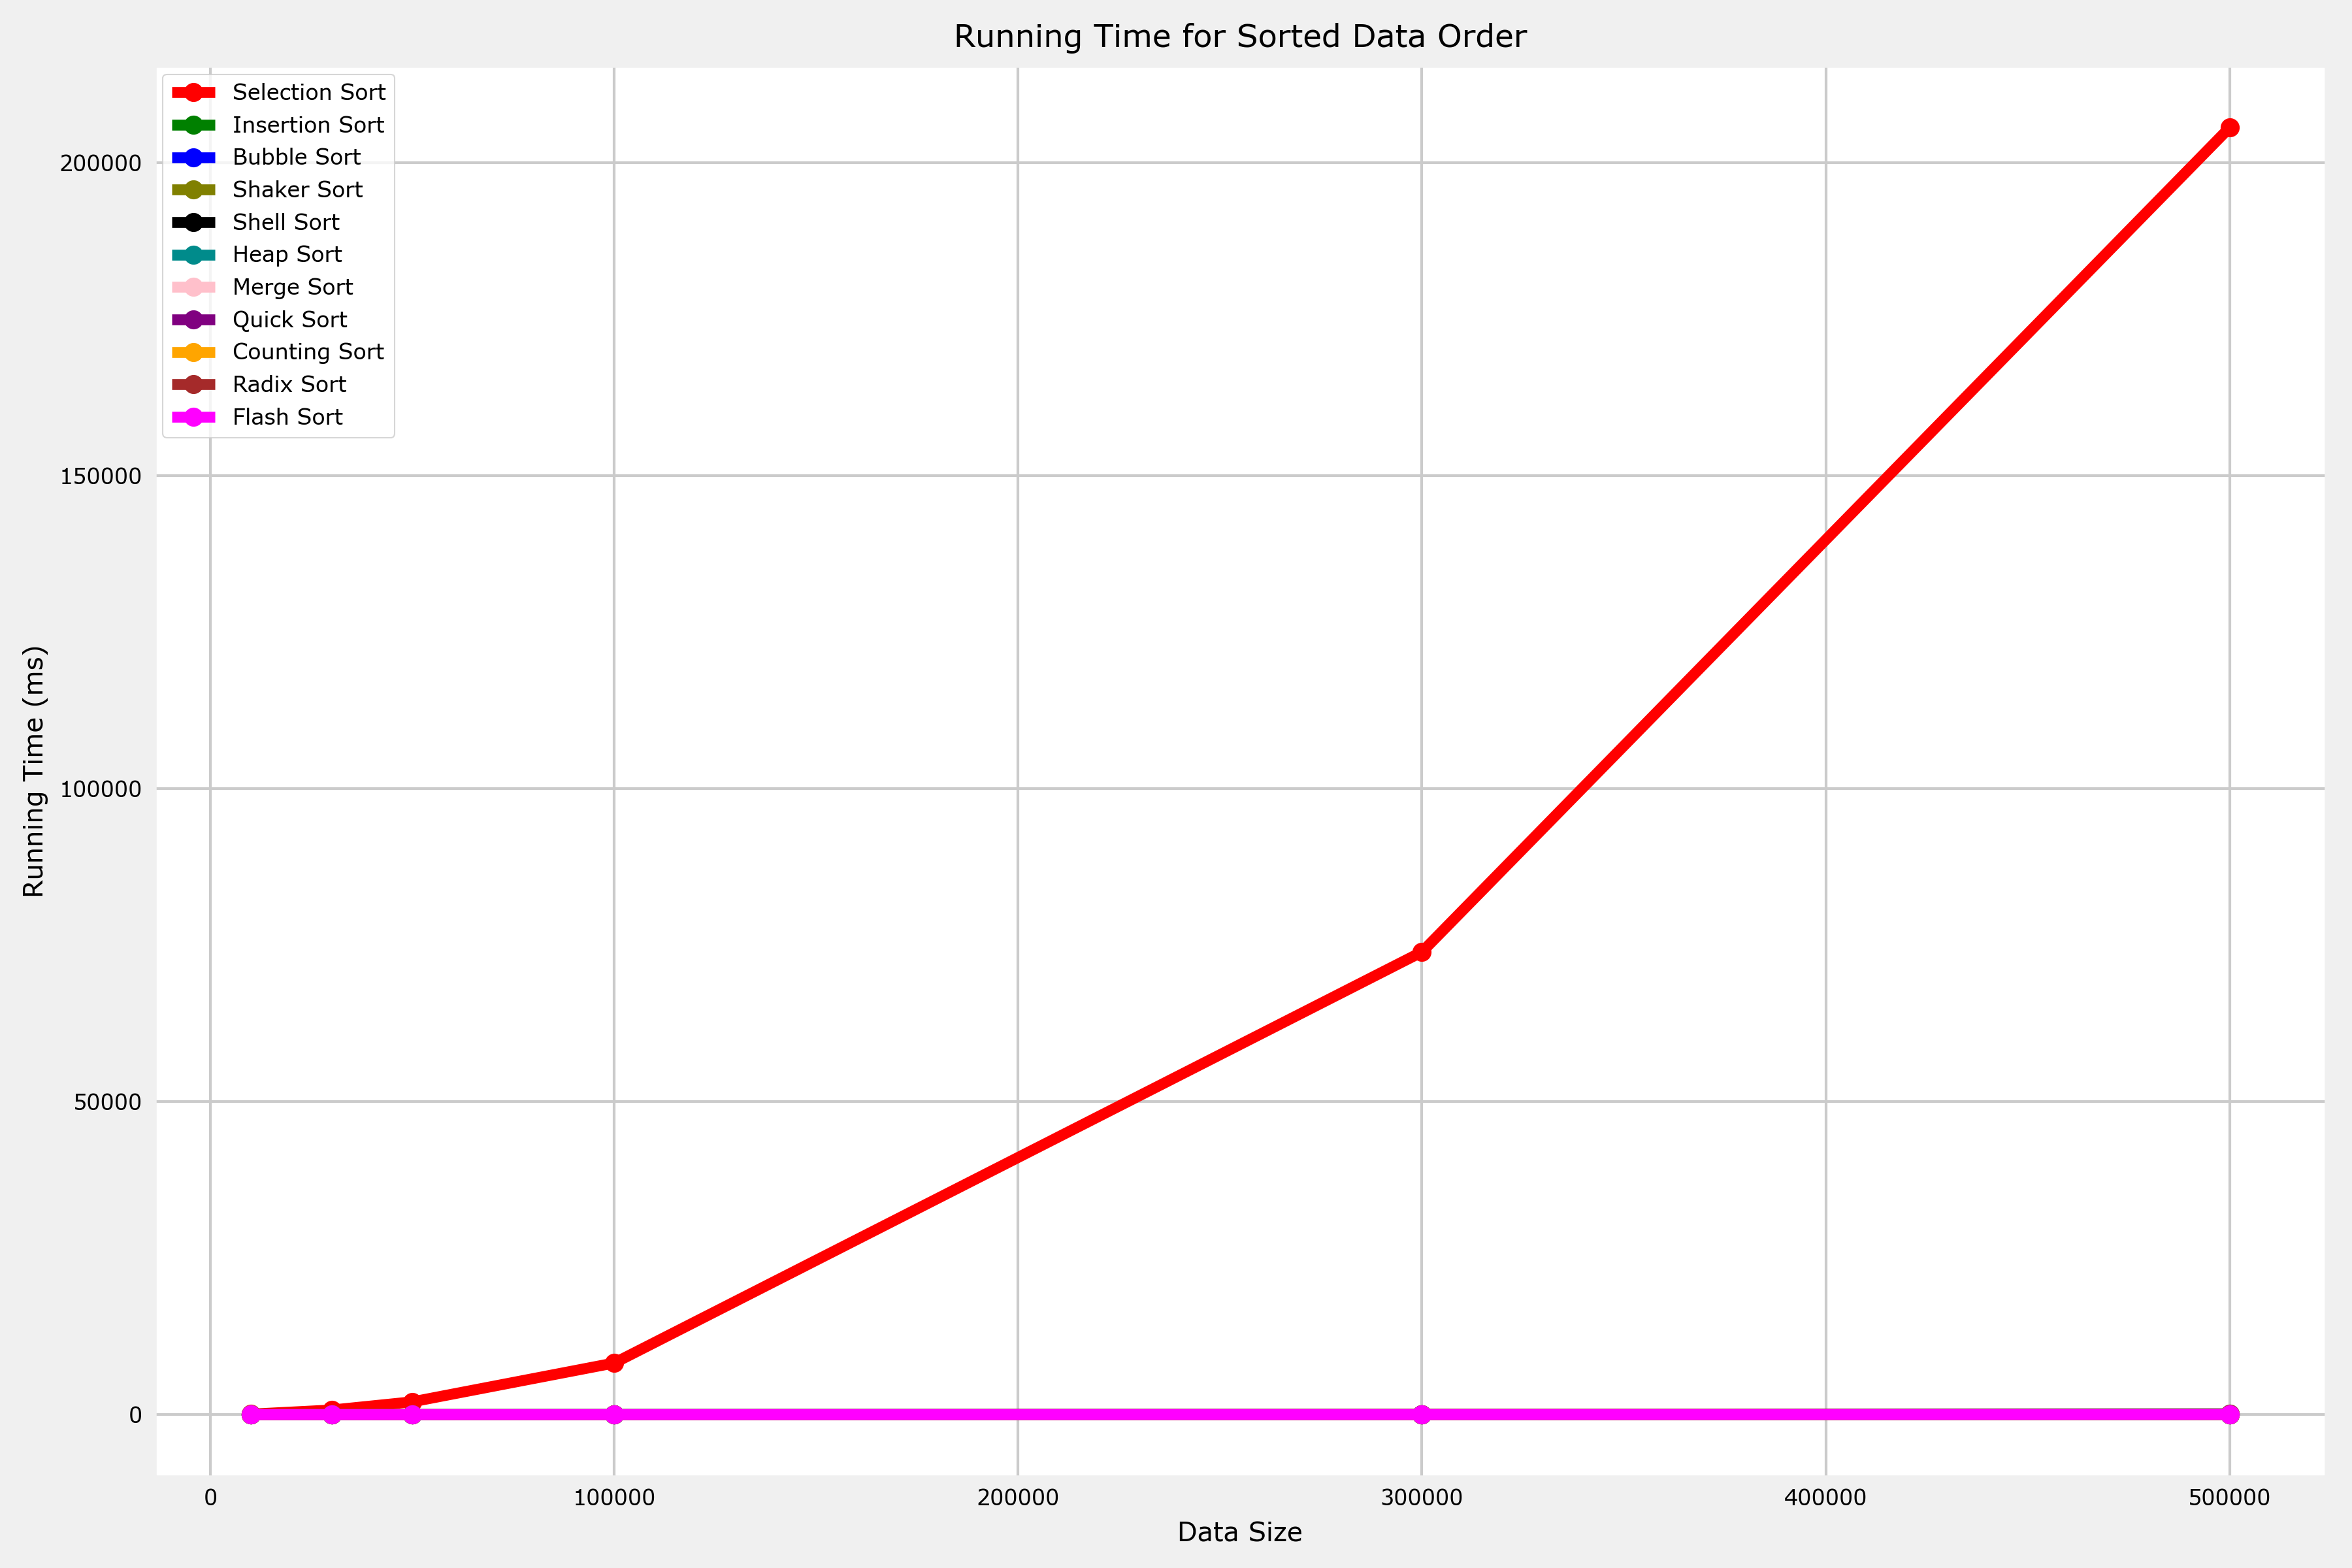
\includegraphics[width=\textwidth]{experimental_result/images/sorted_running_time.png}
    \caption{Thời gian chạy của 11 thuật toán với dữ liệu được sắp xếp}
    \label{fig:sorted_running_time}
\end{figure}

\textbf{3.2.1.3. Dữ liệu được sắp xếp}

Selection vẫn có thời gian thực thi lớn so với các thuật toán còn lại như trên hình \ref{fig:sorted_running_time}. Tiếp tục tách Selection Sort ra khỏi biểu đồ.

\begin{figure}[H]
    \centering
    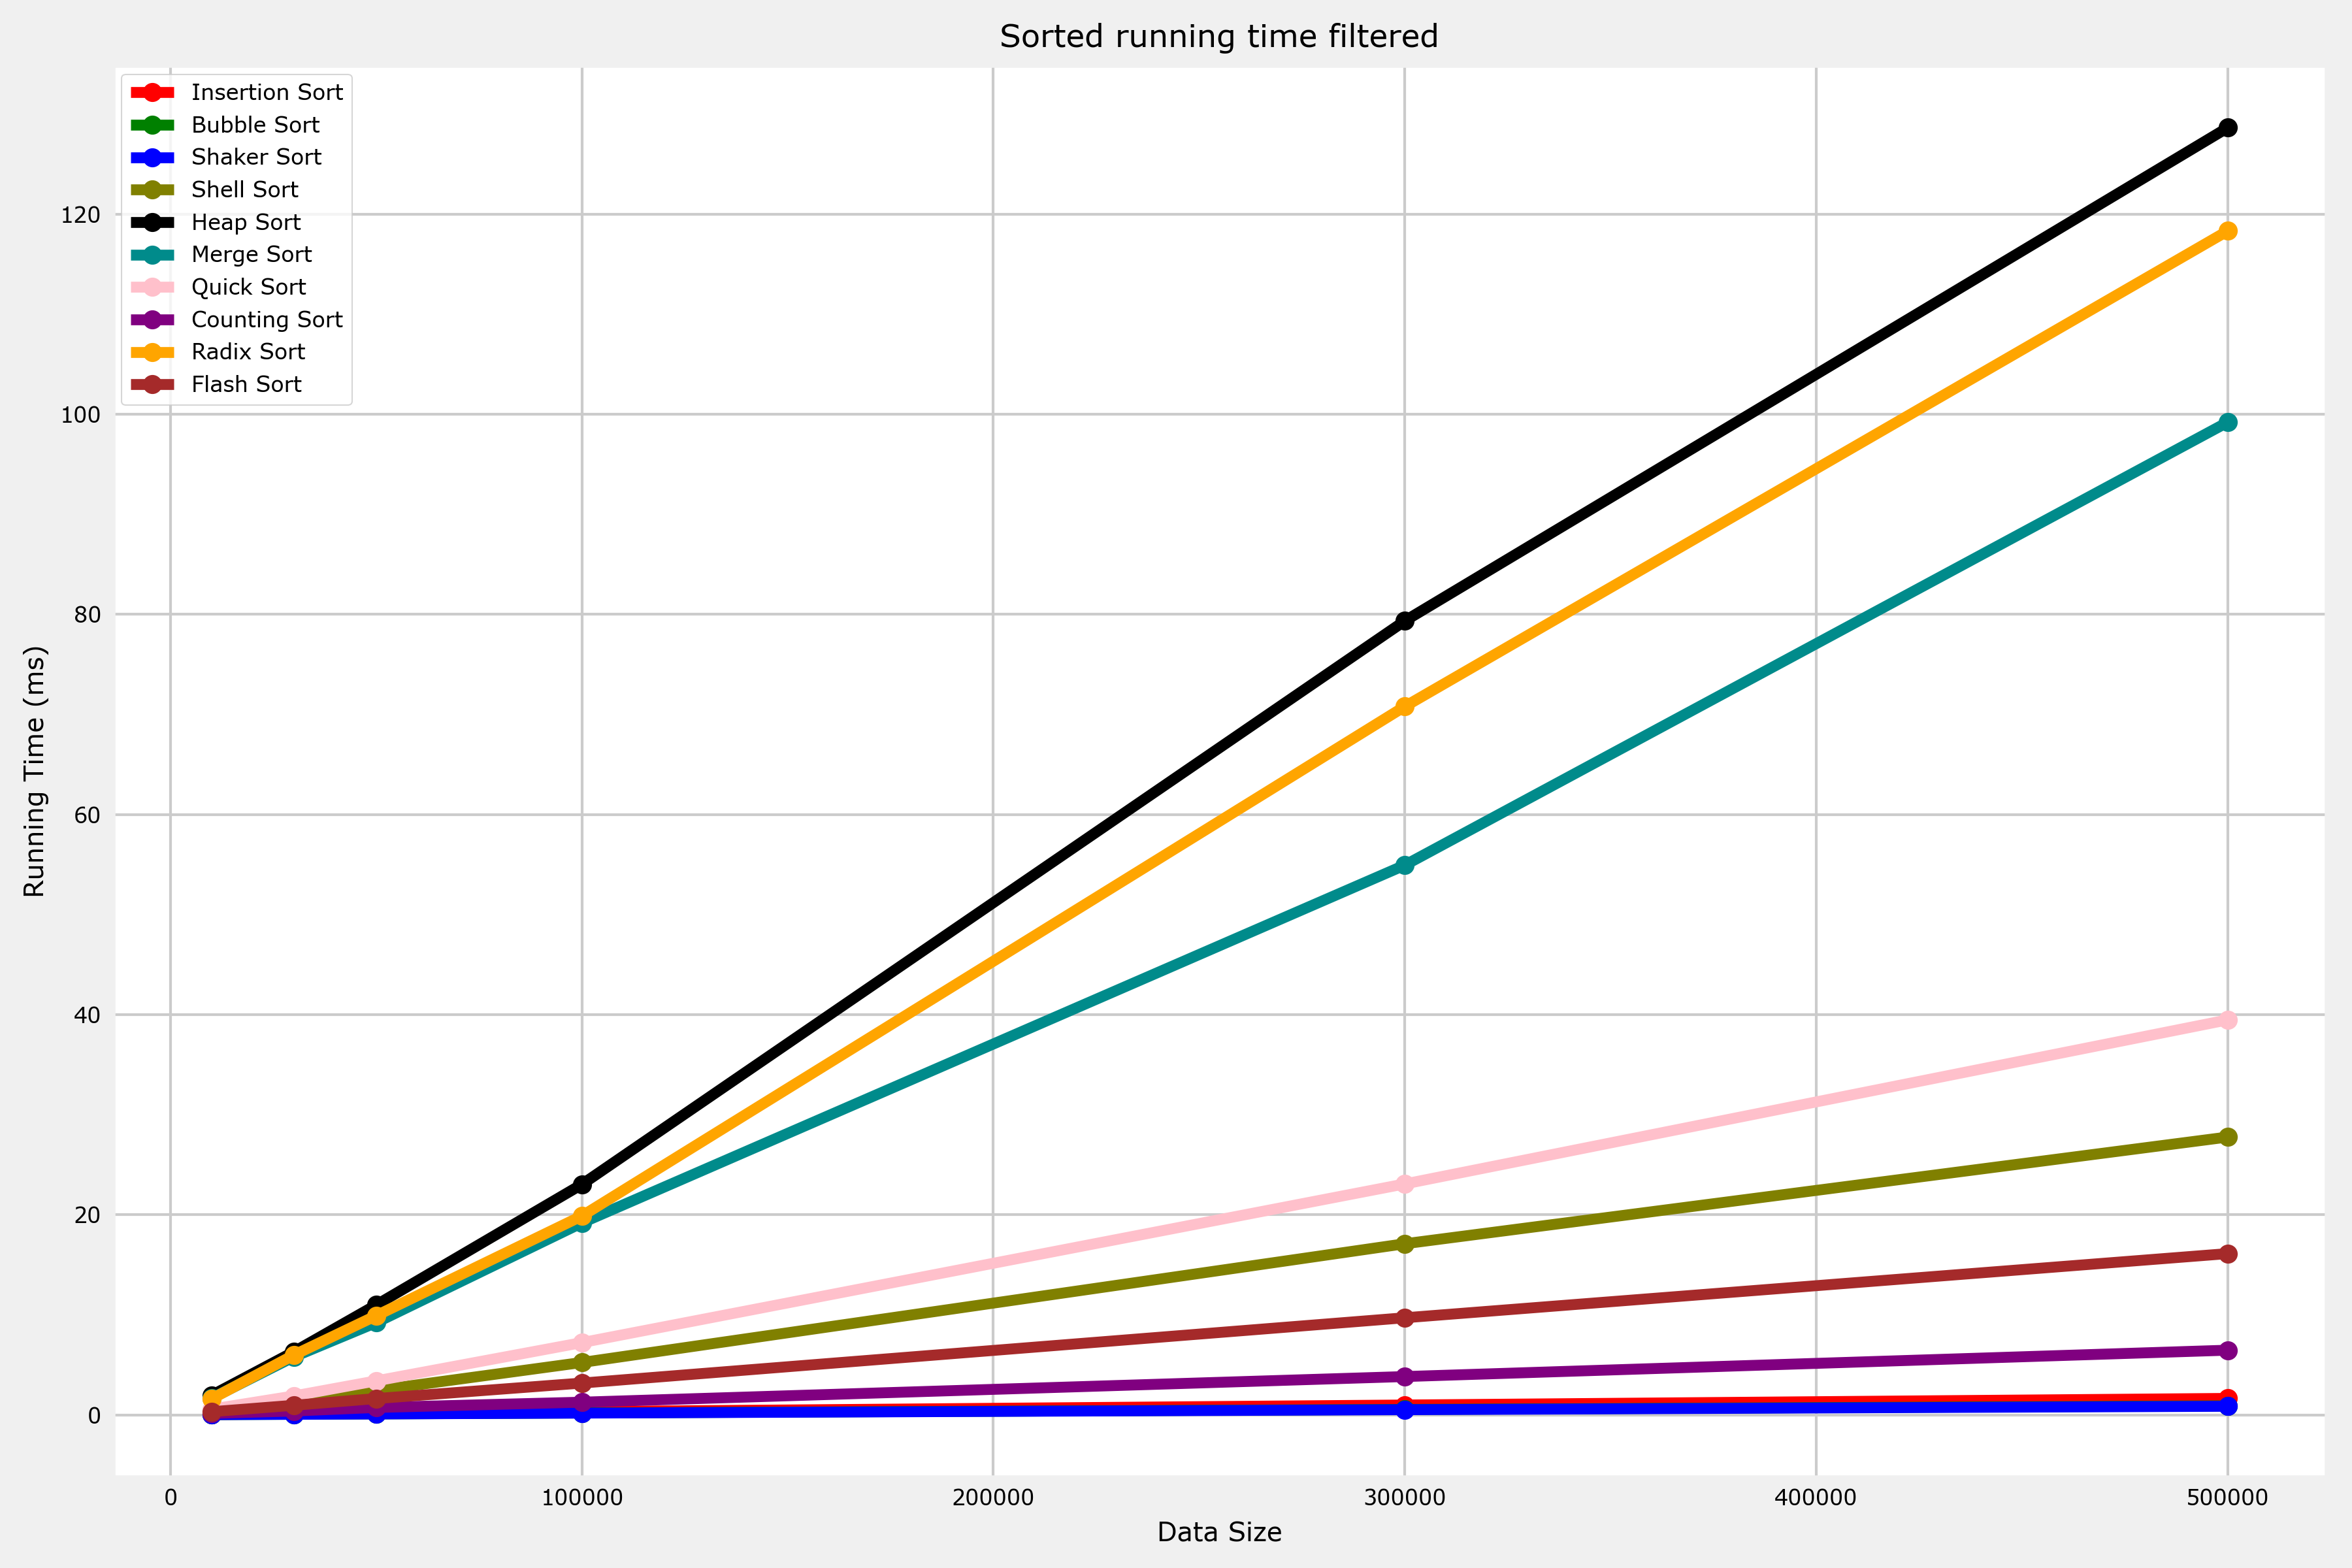
\includegraphics[width=\textwidth]{experimental_result/images/sorted_running_time_filtered.png}
    \caption{Thời gian chạy của 11 thuật toán với dữ liệu được sắp xếp sau khi loại bỏ outlier}
    \label{fig:sorted_running_time_filtered}
\end{figure}

Có hai nhóm thuật toán chính trên biểu đồ \ref{fig:sorted_running_time_filtered}: nhóm 1 (Heap Sort, Radix Sort, Merge Sort) và nhóm 2 (các thuật toán còn lại). Nhóm 1 vẫn giống như trên bộ dữ liệu gần sắp xếp hoàn chỉnh, tương đối ổn định. Nhóm 2 có tốc độ tăng thời gian chạy theo của kích thước của dữ liệu chậm hơn so với nhóm 1. Shaker Sort và Insertion Sort là hai thuật toán nhanh nhất. Bộ dữ liệu này chính là trường hợp tốt nhất cho độ phức tạp thời gian của hai thuật toán này và bằng $\Theta(n)$.


\begin{figure}[H]
    \centering
    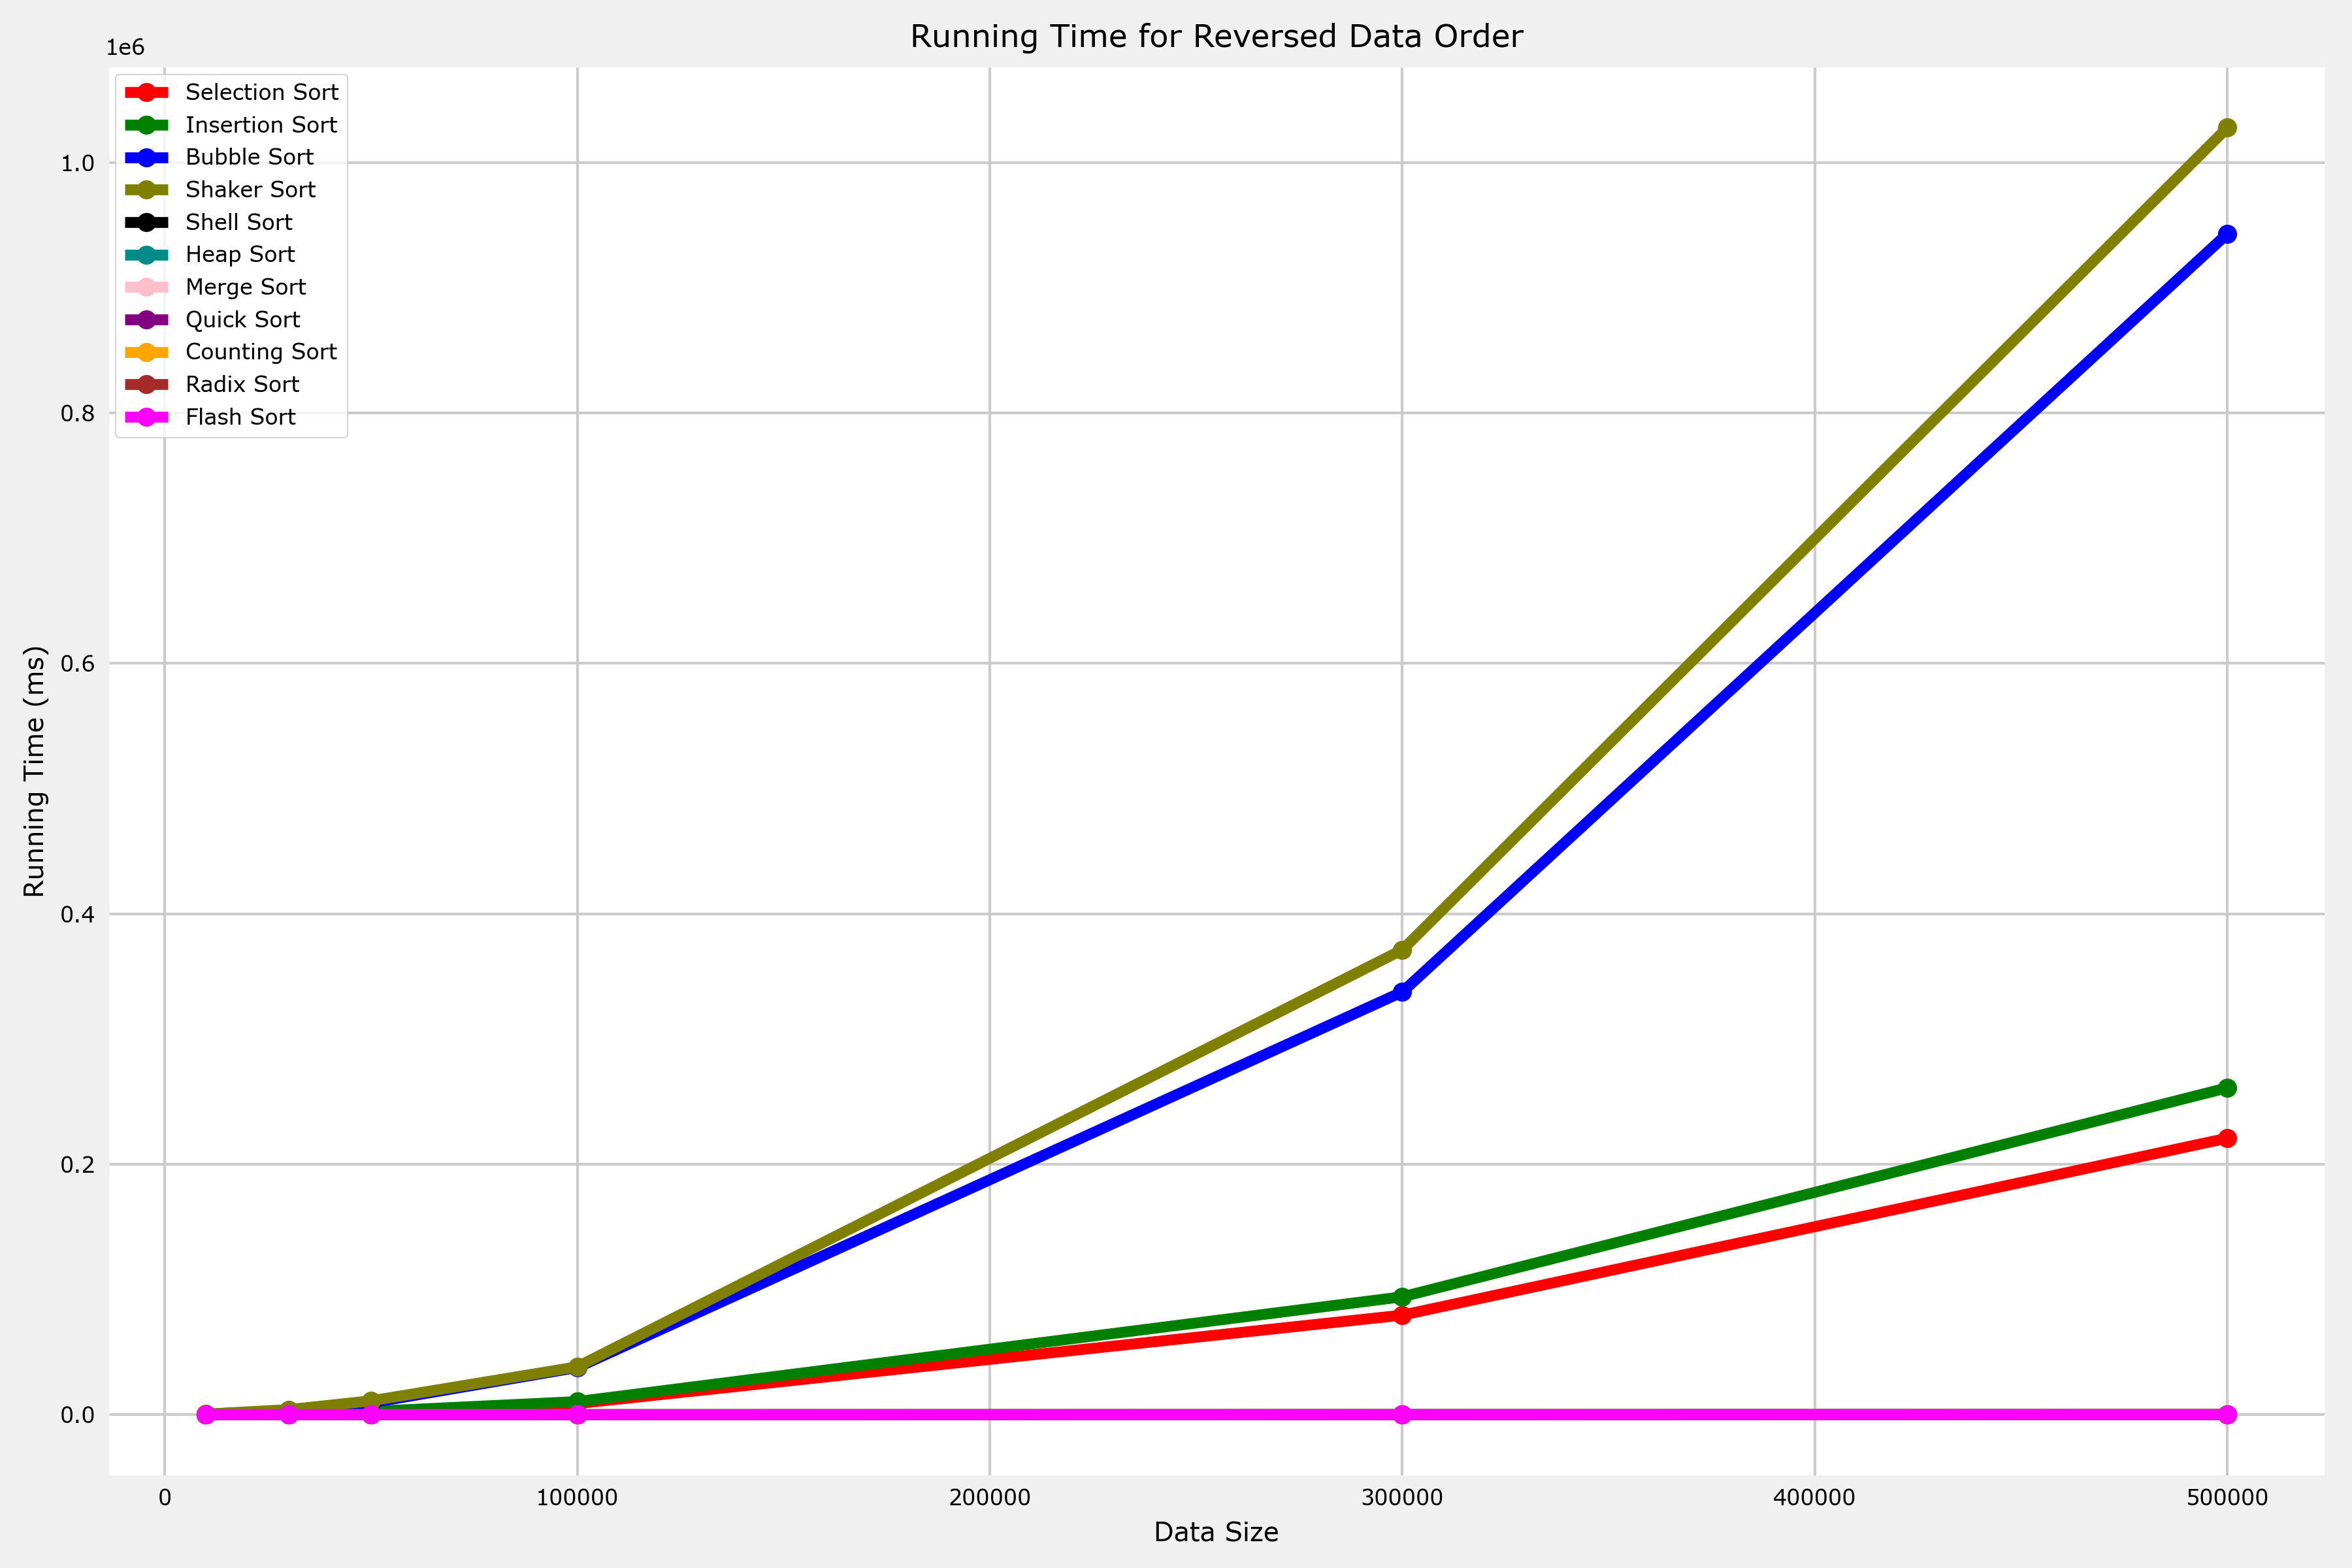
\includegraphics[width=\textwidth]{experimental_result/images/reversed_running_time.png}
    \caption{Thời gian chạy của 11 thuật toán với dữ liệu đảo ngược}
    \label{fig:reversed_running_time}
\end{figure}

\textbf{3.2.1.4. Dữ liệu đảo ngược}


Đối với bộ dữ liệu đảo ngược, Shaker Sort có thời gian chạy tương đối bằng Bubble Sort. Thời gian thực thi của Selection Sort và Insertion Sort khá giống nhau. Shaker Sort và Bubble Sort thể hiện khuynh hướng tăng mạnh hơn so với Selection Sort và Insertion Sort khi gặp kích thước dữ liệu lớn. Hình \ref{fig:reversed_running_time_filtered} có được sau khi bỏ qua 4 thuật toán nhóm cơ bản.

\begin{figure}[H]
    \centering
    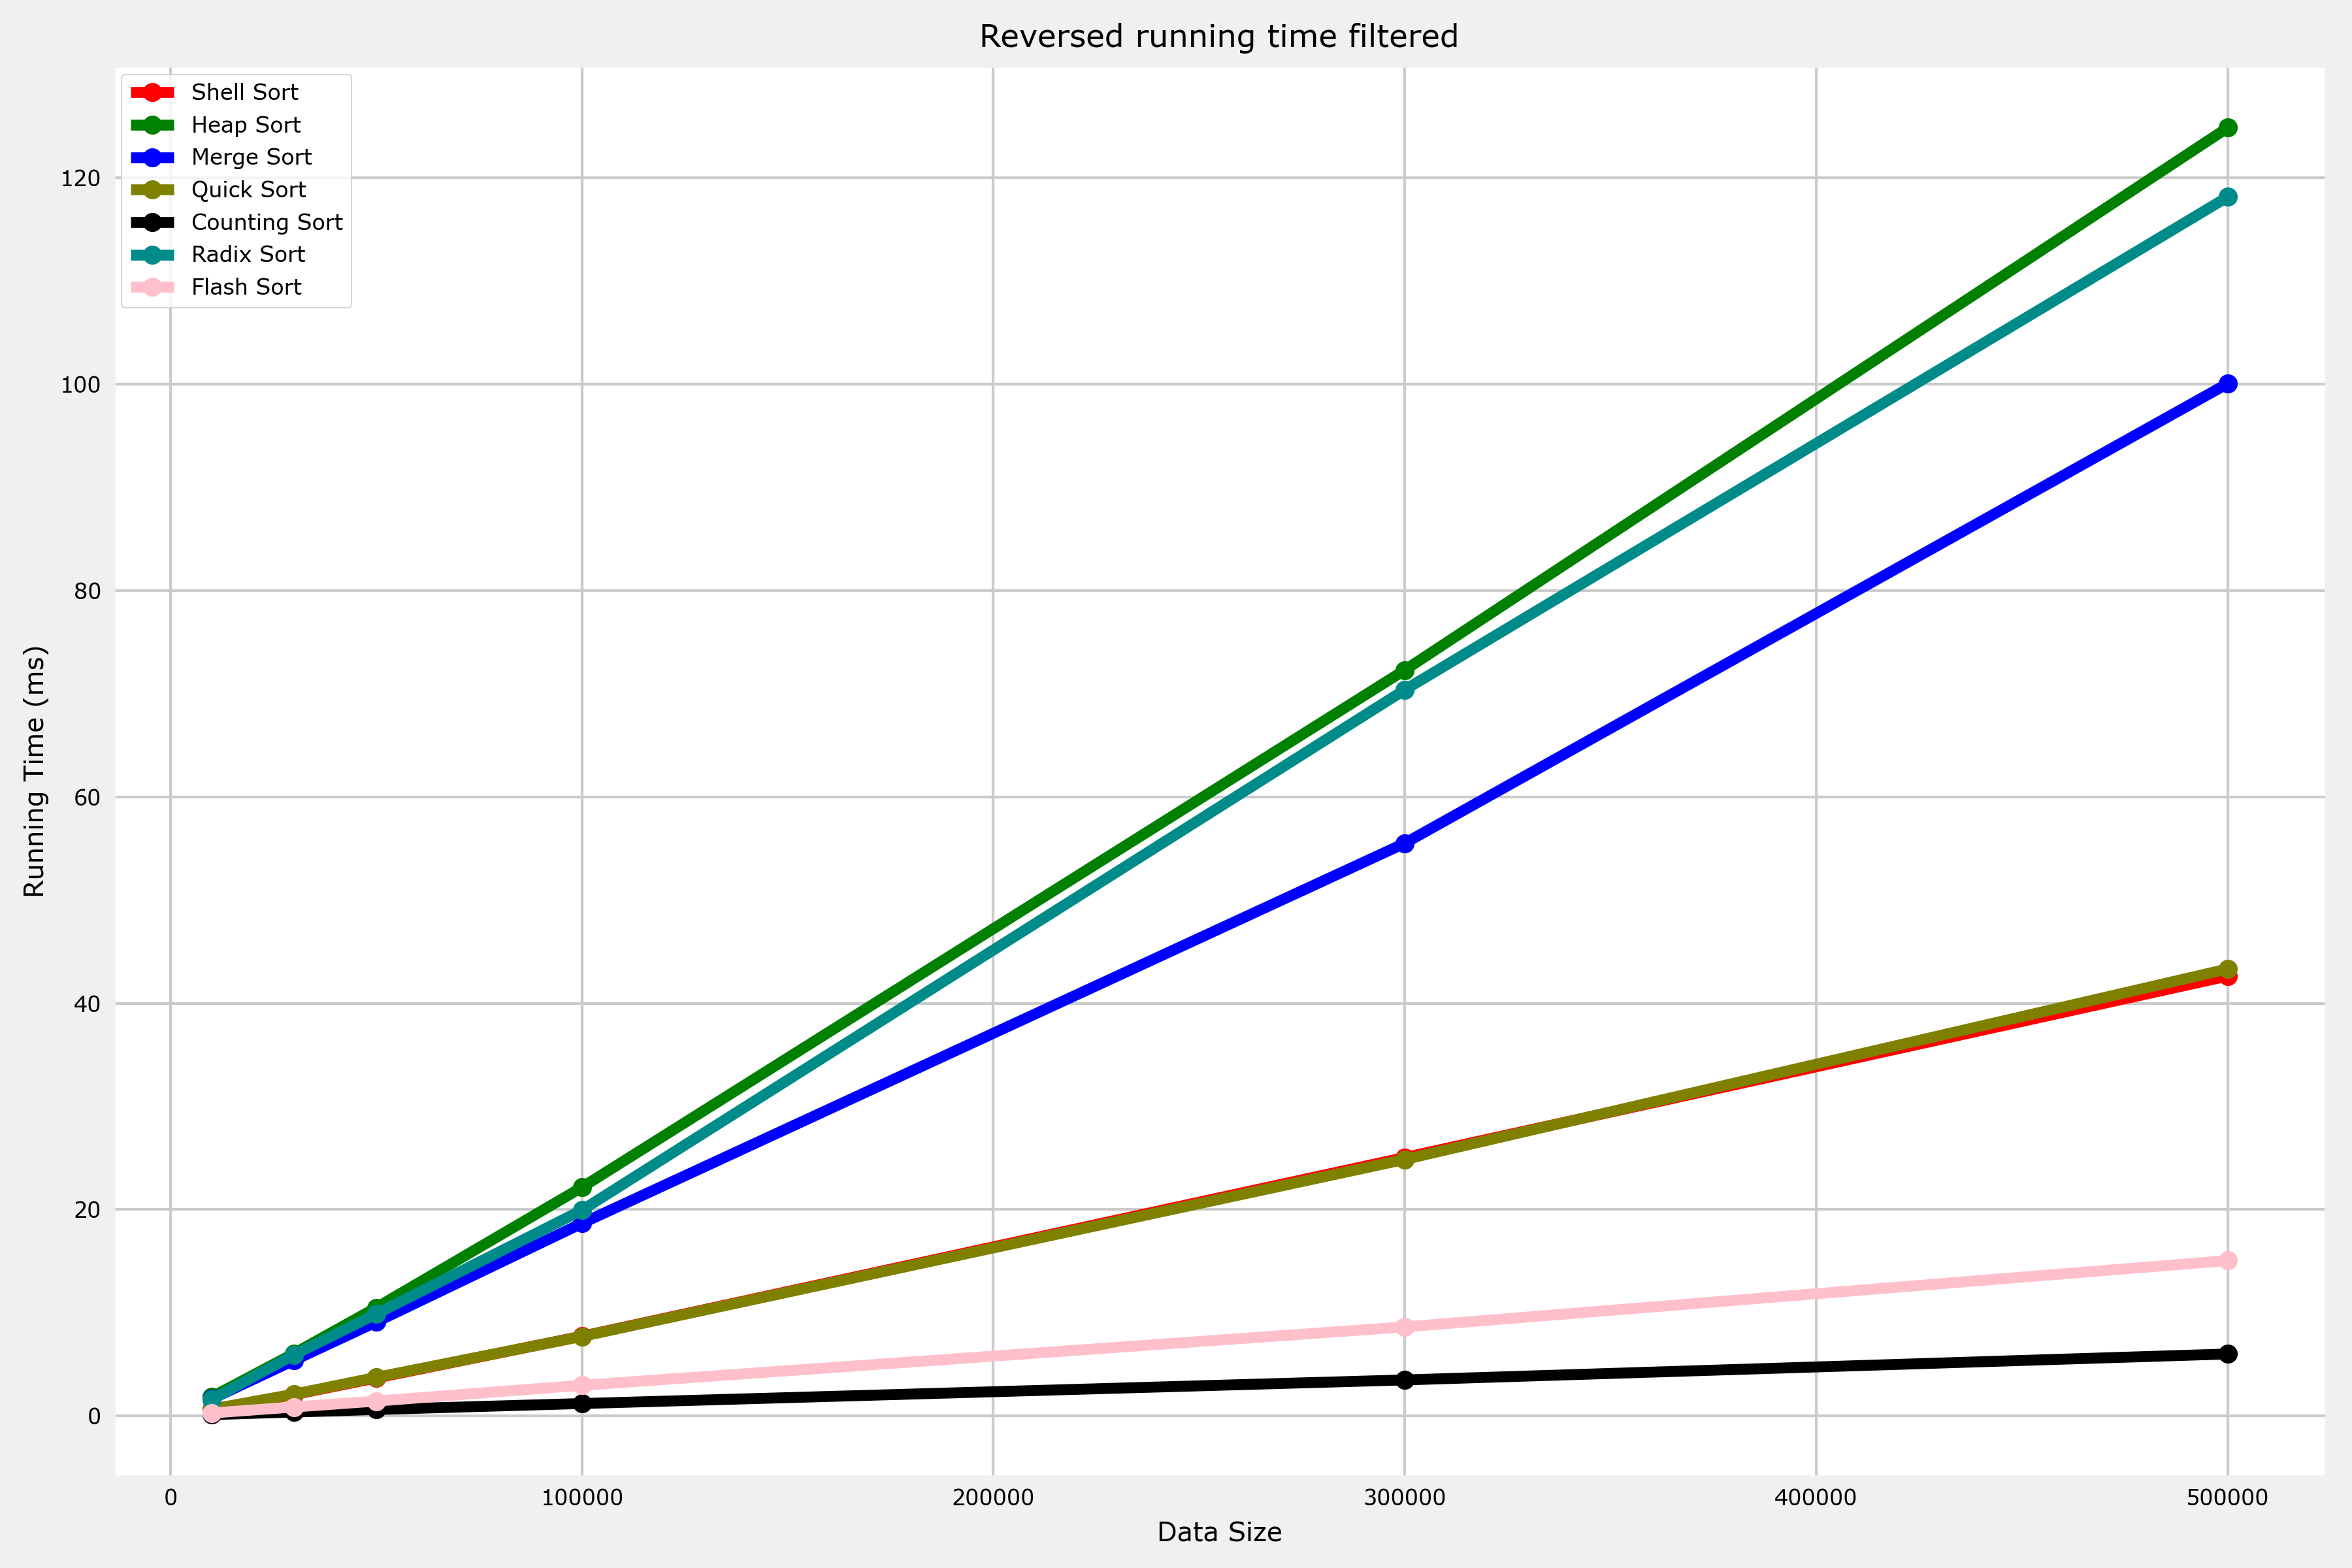
\includegraphics[width=\textwidth]{experimental_result/images/reversed_running_time_filtered.png}
    \caption{Thời gian chạy của 11 thuật toán với dữ liệu đảo ngược sau khi loại bỏ outlier}
    \label{fig:reversed_running_time_filtered}
\end{figure}


Ba thuật toán Heap Sort, Radix Sort, Merge Sort đã thể hiện được tính ổn đỉnh trong cả tất cả trường hợp. Hai thuật toán nhanh nhất vẫn là Counting Sort và Flash Sort. Đường biểu diễn của Quick Sort và Shell Sort khá trùng nhau.







